\documentclass[11pt]{amsbook}

\usepackage{../HBSuerDemir}	
\usepackage[utf8]{inputenc}
\usepackage{amsmath}
\usepackage{mathtools}
\usepackage{graphicx,wrapfig,lipsum}
\usepackage{textcomp}



\begin{document}

% ++++++++++++++++++++++++++++++++++++++
\hPage{b1p2/315}
% ++++++++++++++++++++++++++++++++++++++


\begin{align*}
	\Rightarrow & 2 + 3 sin \Theta  = 0      \\
	\Rightarrow & tan \Theta = \frac{\sqrt{5}}{2} 
\end{align*}

\begin{align*}
     2a &  = \left | BB' \right | = 8 \Rightarrow a = 4, \\ 
     c  &  = ae = 6 \hspace{1cm} b = \sqrt {36 - 16} = 2\sqrt 5 \\
    \left | MH \right |& = a/e = 8/3, \hspace{0.5cm} \left | MF \right | = ae = 6
\end{align*}

 
 
The following two subjects (limo\c{c}ons of PASCAL and curves of CASSINI) are given in some detail, but for the reader not interested in the details, their equations and shape of the curves may be important.


%\underline{Limo\c{c}ons of PASCAL}
Limo\c{c}ons of PASCAL


These curves are defined as follows: 


Consider a circle (center at C) of diameter $\delta$ and a fixed point 0 on it, and consider a line through the fixed point 0 meeting the circle again at a point M.
\begin{wrapfigure}{r}{4cm}
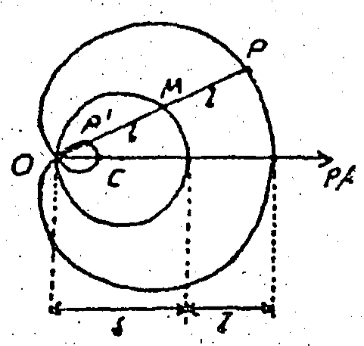
\includegraphics[width=3.5cm]{images/b1p2-315.png}
\end{wrapfigure} 
On this line lay-off segments (MP), (MP\textquotesingle) of constant length 2.


When the point M describes the circle, the points P describe a closed curve called a \textit{limo\c{c}ons of PASCAL} or simply a \textit{limo\c{c}ons}.


To obtain the polar equation of this limo\c{c}ons, we choose the fixed point 0 as pole and the line OC as polar axis.


The equation of the locus of P$\left ( \Theta , r \right )$ is


\begin{equation}\tag{1}
\label{eq:first}
r = l  + \delta cos\theta 
\end{equation}
while that of P\textquotesingle $ \left ( \Theta , r \right )  $ is 
\begin{equation}\tag{1'}
\label{eq:second}
r = - l  + \delta cos\theta
\end{equation}
Since \eqref{eq:second} can be obtained from \eqref{eq:first} by changing $\theta$ to $\theta + \pi$ and r
\end{document}